\documentclass{article}

\usepackage{tikz}
\usetikzlibrary{shapes.geometric,er,positioning}

\usepackage{minted}

\title{
    15-415/615 - Database Applications

    Answers to Homework 1
}
\author{Shangning Xu}

\begin{document}

\maketitle

\section*{Question 1: Entity-Relationship Diagram}

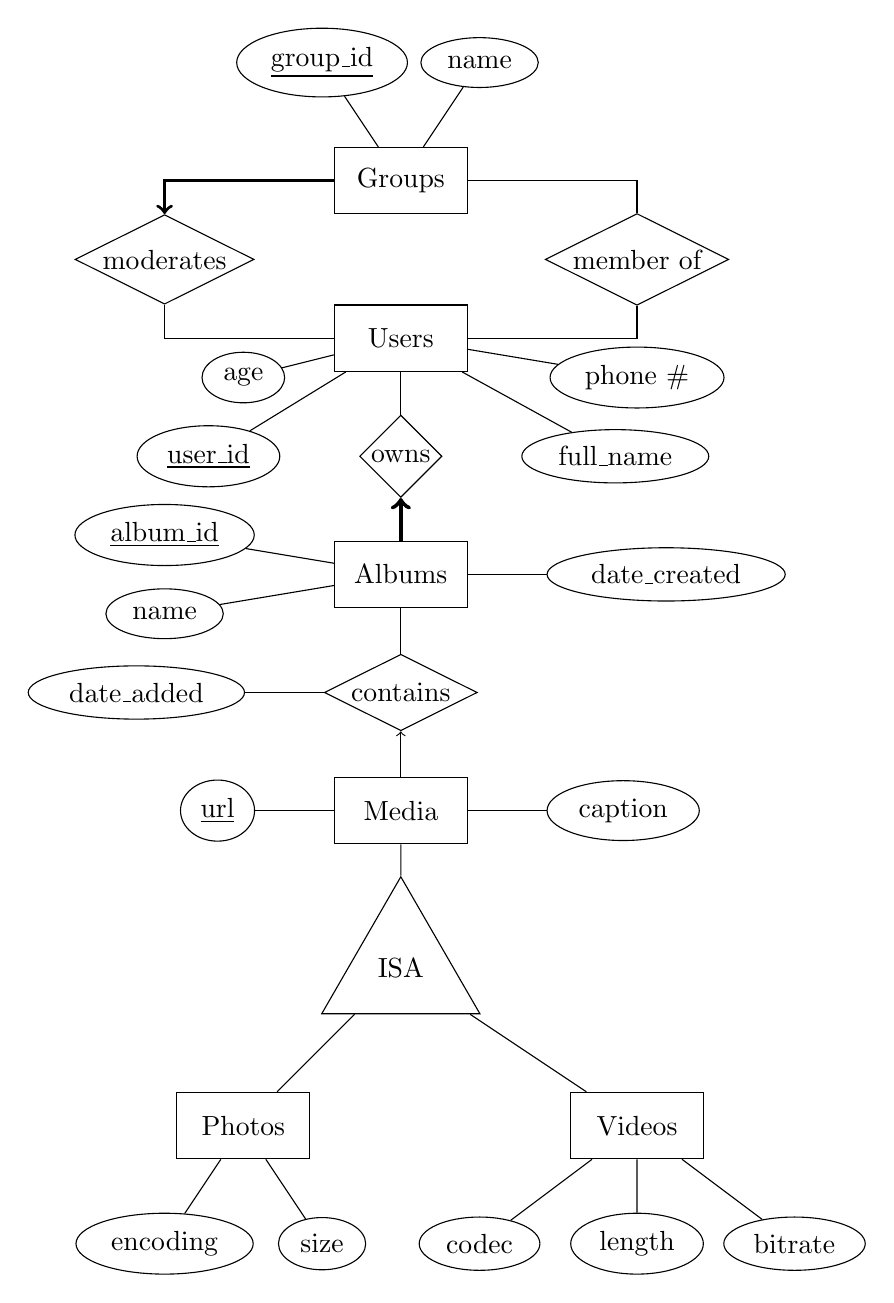
\begin{tikzpicture}
    \node (photos) at (1, 1) [entity] {Photos} [sibling distance=20mm]
        child {node [attribute] {encoding}}
        child {node [attribute] {size}};
    \node (videos) at (6, 1) [entity] {Videos} [sibling distance=20mm]
        child {node [attribute] {codec}}
        child {node [attribute] {length}}
        child {node [attribute] {bitrate}};

    \node (isa) at (3, 3)
        [regular polygon, regular polygon sides=3, draw] {ISA}
        edge (photos) edge (videos);

    \node (media) at (3, 5) [entity] {Media} edge (isa);
    \node (url) [attribute, left=of media] {\underline{url}}
        edge (media);
    \node (caption) [attribute, right=of media] {caption}
        edge (media);

    \node (contains) at (3, 6.5) [relationship, aspect=2] {contains}
        edge [<-] (media);
    \node (date added) [attribute, left=of contains] {date\_added}
        edge (contains);

    \node (albums) at (3, 8) [entity] {Albums} edge (contains);
    \node (album id) at (0, 8.5) [attribute] {\underline{album\_id}}
        edge (albums);
    \node (name) at (0, 7.5) [attribute] {name} edge (albums);
    \node (date created) [attribute, right=of albums] {date\_created}
        edge (albums);
    
    \node (owns) at (3, 9.5) [relationship] {owns}
        edge [<-, ultra thick] (albums);

    \node (users) at (3, 11) [entity] {Users} edge (owns);
    \node (user id) [attribute, left=of owns] {\underline{user\_id}}
        edge (users);
    \node (full name) [attribute, right=of owns] {full\_name} edge (users);
    \node (age) at (1, 10.5) [attribute] {age} edge (users);
    \node (phone) at (6, 10.5) [attribute] {phone \#} edge (users);

    \node (groups) at (3, 13) [entity] {Groups} [grow'=up, sibling distance=20mm]
        child foreach \mytext in {\underline{group\_id}, name}
            {node [attribute] {\mytext}};
    \node (moderates) at (0, 12) [relationship, aspect=2] {moderates};
    \draw [<-, very thick] (moderates) |- (groups);
    \draw (moderates) |- (users);

    \node (member of) at (6, 12) [relationship, aspect=2] {member of};
    \draw (groups) -| (member of) |- (users);
\end{tikzpicture}

\newpage

\section*{Question 2: SQL Tables from the ER Model}

\begin{minted}[linenos]{sql}
CREATE TABLE Buildings (
    building_id INTEGER NOT NULL,
    name CHAR (64),
    date_built DATE,
    PRIMARY KEY (building_id)
)

CREATE TABLE ApartmentUnits (
    unit_id INTEGER NOT NULL,
    n_rooms INTEGER,
    sq_footage REAL,
    building_id INTEGER NOT NULL,
    PRIMARY KEY (unit_id),
    FOREIGN KEY (building_id) REFERENCES Buildings ON DELETE CASCADE
)

CREATE TABLE Tenants (
    tenant_id INTEGER NOT NULL,
    name CHAR(128),
    unit_id INTEGER NOT NULL,
    from_date DATE,
    to_date DATE,
    rent REAL,
    PRIMARY KEY (tenant_id),
    FOREIGN KEY (unit_id) REFERENCES ApartmentUnits ON DELETE CASCADE
)

CREATE TABLE TenantFriends (
    tenant_a_id INTEGER NOT NULL,
    tenant_b_id INTEGER NOT NULL,
    PRIMARY KEY (tenant_a_id, tenant_b_id),
    FOREIGN KEY (tenant_a_id) REFERENCES Tenants.tenant_id
        ON DELETE CASCADE,
    FOREIGN KEY (tenant_b_id) REFERENCES Tenants.tenant_id
        ON DELETE CASCADE
)
\end{minted}

\end{document}
